\documentclass[tcc]{ic}


\usepackage{collectbox}

\makeatletter
\newcommand{\mybox}{%
    \collectbox{%
        \setlength{\fboxsep}{2pt}%
        \fbox{\BOXCONTENT}%
    }%
}
\makeatother

%%%%%%%%%%%%%%%%%%%%%%%%%%%%%%%%%%%%
\hypersetup{
colorlinks = {true},
linktocpage = {false},
plainpages = {false},
linkcolor = {black},
citecolor = {Blue},
urlcolor = {Red},
unicode = {true},
pdftitle = {TCC DUDA},
pdfauthor = {Eduarda Tatiane Caetano Chagas},
pdfsubject = {Relatório Final de Projeto de Iniciação Científica},
pdfkeywords={Teoria da Informação, Séries Temporais, linguagem de programação R},
pdfcreator = {LaTeX2e},
pdffitwindow = {false},
pdfstartview = {FitH},
pdftoolbar = {true},
pdfpagemode = {UseOutlines},
pdfview = {XYZ null null null}
}
%%%%%%%%%%%%%%%%%%%%%%%%%%%%%%%%%%%%%

\titulo{Teoria da Informação e Estatística Computacional no Processamento e Análise de Sinais -- Uma ferramenta para Análise de Séries Temporais}

\autor{Eduarda Tatiane Caetano Chagas}{eduardachagas48@laccan.ufal.br}{}

\orientador{Prof.\ Dr.\ Alejandro Cesar Frery Orgambide}{}{Instituto de Computação}{Universidade Federal de Alagoas}

\examinador{}

\examinadorDois{}

\dataMesAno{Outubro}{2018}

\begin{document}

\selectlanguage{portuguese}

\capa

\begin{resumo}

A análise de séries temporais é classicamente feita ou no domínio do tempo ou em algum domínio transformado (Fourier, Wavelet etc.).
Mais recentemente, apareceram técnicas não-paramétricas e, dentre elas, a análise de descritores causais.
Essas técnicas tem como grande vantagem a relativa pouca sensibilidade a perturbações dos dados, e a capacidade de revelar propriedades importantes da dinâmica subjacente ao processo.
A análise dos descritores causais de uma série temporal possui uma ampla aplicabilidade em nossa rotina, por exemplo na análise de ações bancárias, no registro do comportamento da maré, nos índices da taxa de desemprego, nas temperaturas máximas e mínimas diárias de uma cidade, dentre outras incontáveis finalidades. 
Desse modo, relatamos aqui o processo de desenvolvimento de uma plataforma de análise dos descritores causais de uma série temporal oriundos da Teoria da Informação.
A plataforma visa facilitar a análise dessas séries nos mais variados ramos da ciência. 
O sistema foi implementado na linguagem de programação \texttt R que, além de fornecer ferramentas gráficas, também possui uma grande precisão numérica, ambas características de extrema importância ao longo deste trabalho.

\vspace{2em}
\textbf{Palavras-chave}: Séries Temporais; Teoria da Informação; Linguagem \texttt R.

\end{resumo}

\selectlanguage{english}
\begin{abstract}

Time series analysis is classically performed either in the time domain or in a transformed domain (Fourier, Wavelet, etc.)
More recently, nonparametric techniques have been proposed and, among them, the use of time causal descriptors.
This class of techniques has the ability to reveal important properties of the underlying process and, at the same time, to be relatively insensitive to data contamination.
The analysis of causal descriptors of a time series has a wide applicability, as in the analysis stock market, records of the behavior of the tides, index of the unemployment rates, maximum and minimum daily temperatures of a city, among others.
We report here the process of developing a platform for analyzing causal descriptors of a time series using Information Theory.
The platform aims to facilitate the analysis of such series in as many branches of science as possible.
The system was implemented in the \texttt R programming language, which besides providing graphical tools, also has a great numerical precision, both features of extreme importance throughout this work.

\vspace{2em}
\textbf{Keywords}: Time Series; Information Theory; Language \texttt R;

\end{abstract}

\selectlanguage{portuguese}

\tableofcontents

\listoffigures
\addcontentsline{toc}{table}{Lista de Figuras}

\listoftables
\addcontentsline{toc}{table}{Lista de Tabelas}

\inicio

\mychapter{Introdução}{cap:introducao} \lhead{INTRODUÇÃO}

\section{Motivação}

Séries temporais estão presentes em todo o nosso cotidiano. Sendo definidas como um conjunto de dados obtidos a partir de um processo observacional ao longo de um determinado período de tempo, não necessariamente dividido em espaços iguais, estes dados são caracterizados pela dependência serial existente entre as observações.

A hipótese subjacente a toda essa análise é que os dados observados são o resultado da operação de um sistema causal sujeito a ruído observacional. Logo, esse sistema, ou dinâmica, é responsável pela criação de padrões através de cuja observação deseja-se inferir a respeito da dinâmica. Portanto, o estudo de tais dados auxilia na análise de diversas propriedades de sistemas. 

Como comentado anteriormente, a aplicação deste conhecimento pode ser encontrada em múltiplas áreas do conhecimento científico como, por exemplo, 
na discriminação entre fenômenos estocásticos e caóticos~\cite{DistinguishingNoiseFromChaos}, 
na identificação de padrões de comportamento em redes veiculares~\cite{CharacterizationVehicleBehaviorInformationTheory}, 
na classificação e verificação de assinaturas \textit{online} ~\cite{ClassificationVerificationOnlineHandwrittenSignatures},
na análise da eficiência informacional do mercado de petróleo~\cite{oilMarket},
na caracterização das séries temporais produzidas por eletroencefalogramas~\cite{EGGTimeSeries},
na análise da robustez de redes~\cite{InformationTheoryPerspectiveNetworkRobustness}, e 
na classificação de padrões de consumo de energia elétrica~\cite{CharacterizationElectricLoadInformationTheoryQuantifiers}.

Tradicionalmente o estudo de séries temporais costuma ser dividido em duas linhas de estudo, nos domínios do tempo e da frequência~\cite{BrockwellDavis91}. No entanto, ambas abordagens utilizam diretamente os dados resultantes do processo observacional, que são sensíveis a efeitos provocados por diversos tipos de contaminação. Logo, surge assim a abordagem do uso de métodos não paramétricos, como uma forma de evitar que tais efeitos invalidem as análises destes dados.

A Teoria da Informação surgiu como um ramo interdisciplinar, produzindo inúmeros resultados, tanto no ponto de vista teórico quanto nas aplicações, na criação de novos métodos na extração de informações de sinais, abrangendo em suas soluções conceitos presentes na Probabilidade, Estatística, e Telecomunicações. 

O uso de suas ferramentas tem levado a resultados significativamente melhores do que aqueles obtidos com técnicas clássicas em diversas áreas do conhecimento. No trabalho de~\cite{Torres2014}, podemos ver uma grande contribuição no campodo processamento de imagens, onde este propõe uma técnica de filtrado que se adapta a cada ponto da imagem, observa uma janela de tamanho considerável e só emprega aquelas observações que não são muito discrepantes do valor central. Em~\cite{Bhattacharya2015}, vemos uma aplicação de distâncias estocásticas para obter uma decomposição polarimétrica otimizada. Já~ \cite{Gambini2015} propõe uma técnica de estimação de parâmetros minimizando distâncias estocásticas entre modelos e evidência empírica.

Entretanto, diversos desafios surgem na hora de tratar um problema com estes tipos de técnicas, pois ainda existem vários problemas analíticos e de ordem computacional em aberto, formando assim uma linha de pesquisa avançada, uma vez que requerem por parte dos envolvidos um bom domínio das teorias que dão sustento às técnicas.

Atualmente há diversas ferramentas que auxiliam na análise clássica de séries temporais; para a plataforma \texttt  R, existem diversas bibliotecas para essa finalidade (ver \url{https://cran.rproject.org/web/views/TimeSeries.html}). Além destas opções, o usuário também pode contar com os softwares de visualização de séries temporais. No entanto, são limitadas as opções de bibliotecas e softwares que trabalham exclusivamente com técnicas não paramétricas e a sua grande maioria exige familiaridade do usuário com o ambiente utilizado.

Desse modo, exitem dois principais pontos nessas linhas de pesquisa que podem originar ótimos trabalhos inovadores:

\begin{itemize}
\item a necessidade de tornar as técnicas acessíveis a usuários não especializados, e
\item a necessidade de otimizar o desenvolvimento de novas técnicas.
\end{itemize}

O primeiro ponto pode ser solucionado por meio do desenvolvimento de sistemas com interface gráficas que encapsulem os algoritmos presentes na literatura. Já o segundo, consiste em utilizar técnicas de desenvolvimento de software científico.

Logo, é na esfera do domínio dos problemas computacionais que surgem na aplicação de ferramentas oriundas da Teoria de Informação a séries temporais, que este trabalho se insere.
 
Apresentamos, assim, o desenvolvimento de uma ferramenta portável, rápida e de boa qualidade numérica que possibilita análises interativas e exploratórias dos dados de uma série temporal através de técnicas provenientes da Teoria da Informação.
Com ela, o usuário dispõe de uma conjunto técnicas de análise presentes na literatura para processar e examinar seus dados de modo eficiente e com um mínimo período de aprendizado.
A ferramenta é extensível.

\section{Objetivo}

O objetivo geral deste trabalho é propor e desenvolver uma ferramenta inovadora, resultante de propostas recentes de pesquisas relacionadas a Teoria da Informação, para facilitar o uso de técnicas avançadas de processamento e análise de sinais.

\section{Solução proposta}

Realizamos o uso de técnicas modernas de análise de séries temporais. Uma série temporal é transformada em uma sequência de símbolos, através da técnica de simbolização de~\cite{article2}. Essa técnica consiste em transformar vetores de tamanho D em padrões ordinais de forma não-paramétrica e formar um histograma de ocorrência dos D! padrões possíveis. Esse histograma é tratado como uma função de probabilidade, do qual são extraídos descritores oriundos da Teoria da Informação. Esses descritores são, depois, mapeados em um plano adequado, e a sua localização serve para identificar o tipo de dinâmica subjacente à série temporal. Há uma grande diversidade de descritores como, por exemplo, distâncias (Kullback-Leibler, Bhattacharya, Hellinger, Rényi, Triangular, Harmônica, dentre outras), e entropias (Jensen-Shannon, Rényi, Tsallis, dentre outras). O ambiente gráfico oferecerá essas opções, e permitirá experimentar com a sua expressividade.

\section{Contribuições}

As contribuições deste trabalho são:

\begin{itemize}
\item A compreensão e implementação de técnicas de análise não-paramétrica de séries temporais utilizando descritores causais oriundos da Teoria da Informação;
\item A implementação de uma interface gráfica amigável para a aplicação de tais descritores, mantendo a portabilidade do software para os diversos sistemas operacionais e arquiteturas de hardware.
\end{itemize}

Note que essas contribuições podem facilitar este processo de análise e construção do conhecimento por parte do usuário, tornando tal experiência mais simples e completa, fornecendo para este novas funcionalidades, como uma maior interação do gráfico da série com os seus padrões.

\section{Estrutura do texto}

Este trabalho foi dividido em 5 capítulos e um anexo. 
No capítulo~\ref{cap:fundamentacao} introduz algumas das principais técnicas e ferramentas disponíveis na literatura para a análise não-paramétrica de séries temporais utilizando descritores da Teoria da Informação, focando nos conceitos e metodologias aplicados com sucesso em diversos ramos de pesquisa científica.
No capítulo~\ref{cap:metodologia} apresenta a metodologia do trabalho desenvolvido.
No capítulo~\ref{cap:resultados} apresenta os resultados obtidos.
As funções implementadas ao longo do desenvolvimento do projeto se encontram presente no Anexo A.
E, finalmente, no Capítulo~\ref{cap:conclusoes} apresenta as considerações finais, concluindo este trabalho.

\newpage\lhead{\rightmark}

\mychapter{Fundamentação Teórica}{cap:fundamentacao}

Para que se obtenha um melhor entendimento acerca do tema proposto, neste  capítulo  serão  apresentadas  as  fundamentações  teóricas, obtidas por meio da realização da revisão bibliográfica dos conceitos e técnicas presentes no estado da arte.

\section{Representação do espaço de probabilidade}

A transformação de uma série temporal em uma distribuição de probabilidade (PDF) permite avaliar o conteúdo informacional acerca da dinâmica do sistema e dos processos subjacentes, descrevendo-os de forma mensurável e observável~\citep{entropyAndInformationTheory}.
Através desta conversão é possível utilizar métricas do espaço PDF, permitindo comparar diferentes conjuntos e classificá-los de acordo com as propriedades dos processos subjacentes. 
Podemos assim, por exemplo, classificar uma série entre estocástica ou determinística.

A ideia das técnicas não-paramétricas consiste em construir o histograma de algum atributo da série temporal, e extrair dele métricas de Teoria da Informação.
Os atributos são os mais variados~\citep{Kowalski2011DistancesIP}, dentre eles: 
\begin{enumerate}[label=(\alph*)]
\item Padrões ordinais~\citep{ROSSO2},
\item Histogramas~\citep{article3,DEMICCO20083373},
\item Dinâmica simbólica binária~\citep{PhysRevLett},
\item Análise de Fourier~\citep{article}, e 
\item Transformada wavelet~\citep{ROSSO3}. 
\end{enumerate}

Todas estas metodologias são capazes de capturar aspectos globais de dinâmicas complexas. 
No entanto, não é trivial encontrar uma representação simbólica significativa da série original. 
Assim, por considerar a causalidade temporal dos dados, a abordagem de~\citet{article2} revela detalhes importantes da estrutura ordinal da série temporal.

\section{Método de simbolização de Bandt e Pompe }

De acordo com a abordagem de Bandt e Pompe, substituímos a série por sequências de postos, obtidos pela análise desta ao longo do tempo.

Dada uma série temporal a tempo discreto $X = {x_t:1\leq t\leq T}$, uma dimensão $D$ e um tempo de atraso (delay) $\tau$, o particionamento é efetuado por meio da reorganização do sistema em conjuntos seguindo os seguintes passos:

\begin{description}
\item[Composição dos grupos:] A série inicialmente será particionada em conjuntos de tamanho $D$ e delay $\tau$, possuindo a seguinte estrutura: 
		 $$(s) \mapsto (x_{(t-1)+\tau},\ldots, x_{(t-1)+\tau+D-1}).$$  

\item[Formação dos padrões:] Cada grupo formado anteriormente é então relacionado a um padrão ordinal $\pi$ de ordem $D$, como se observa abaixo:
		$$ \{0, 1,\ldots, D-1\}. $$

\item[Elaboração dos símbolos:] É realizada então a permutação dos elementos dos grupos, de tal forma que estes estejam ordenados de forma crescente. 
		$$ x_{(t-1)+\tau} \leq x_{(t-1)+\tau+1} \leq \ldots \leq x_{(t-1)+\tau+D-1}. $$ 
\end{description}

De mesmo modo é impreterível que a permutação ocorra com os elementos dos padrões relacionados a cada grupo, pois estes corresponderam aos símbolos da série. No esquemático da Figura~\ref{fig:patterns} podemos visualizar a relação de cada padrão no comportamento dos elementos da série, sendo perceptível o quanto de informação sobre a estrutura da dinâmica temporal do sistema podemos extrair com essa técnica de simbolização.

\begin{figure}[!ht]
	\begin{center}
		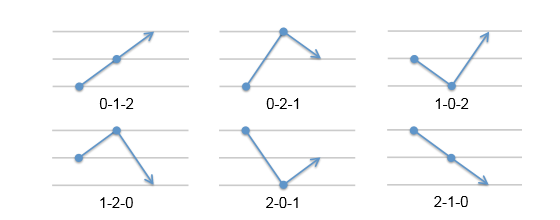
\includegraphics[width=0.6\columnwidth]{capitulos/imagens/padroes.png}
        \caption{Representação gráfica dos padrões com dimensão $D=3$.}
	\label{fig:patterns}
	\end{center}
\end{figure}

A literatura apresenta duas maneiras de definir o mapeamento de padrões~\citep{tiedvalues}:  

\begin{enumerate}[label=(\alph*)]
\item Ordenando as posições dos grupos em ordem cronológica (Permutação de Classificação), e 
\item Ordenando os índices de tempo dos elementos dos subconjuntos (Permutação do Índice Cronológico).
\end{enumerate}

Logo abaixo, observamos como se comporta a representação gráfica dos padrões ordinais quando aplicado cada um desses mapeamentos.

\begin{figure}[!ht]
	\begin{center}
		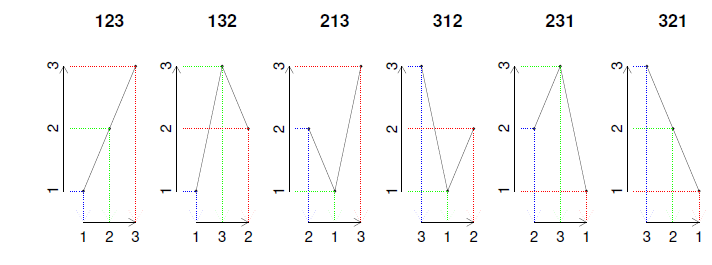
\includegraphics[width=0.7\columnwidth]{capitulos/imagens/rankPermutation.png}
        \caption{Mapeamento por Permutação de Classificação~\citep{tiedvalues}}
	\end{center}
\end{figure}

\begin{figure}[!ht]
	\begin{center}
		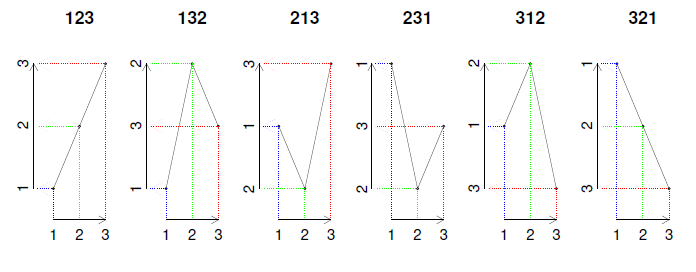
\includegraphics[width=0.7\columnwidth]{capitulos/imagens/chronologicalIndex.png}
        \caption{Mapeamento por Permutação do Índice Cronológico~\citep{tiedvalues}}
	\end{center}
\end{figure}
				
%=========================================================

\section{Distribuição de probabilidade de Bandt e Pompe}

Em estatística, uma distribuição discreta de probabilidade refere-se à distribuição de frequências relativas para os resultados de um espaço amostral, apontando a quantidade de vezes em que um determinado elemento do conjunto assume cada um dos seus possíveis valores.

Logo:
 $$\sum_{n}^{i=1} P_{i} = 1. $$ 

Considerando isto, a distribuição de probabilidade de Bandt \& Pompe consiste no cálculo da distribuição dos símbolos da série diante das $D!$ possíveis permutações dos padrões ordinais $\pi$ de comprimento $D$:

$$p(\pi)=\frac{\left \{\#t | t \leq T- (D-1)\tau    , (x_{t+1}, \ldots, x_{t+D}) \indent do \indent tipo \indent \pi\right \}}{T- (D-1)\tau}  $$ 

Uma grande vantagem de sua utilização refere-se ao fato da distribuição de probabilidade tornar-se invariante com respeito às transformações monotônicas, propriedade extremamente desejada na análise das séries.

Uma vez calculado o histograma de padrões $\bm p=(p_1,\dots,p_{D!})$, isto é, a função de probabilidade, o próximo passo será obter descritores.

\section{Entropia de permutação}

A Entropia mede o desordem ou a imprevisibilidade de um sistema caracterizado por uma função de probabilidade $\bm p$.
Neste trabalho, citaremos três modelos de entropia: Shannon, Tsallis e Rényi.

Proposta em 1948, a entropia de Shannon consiste de uma variação da Entropia de Boltzmann-Gibbs~\citep{shannon}. Seja, assim, $\bm p=(p_1,\dots,p_{D!})$ o histograma de proporções dos $D!$ padrões observados a partir da série temporal $\bm X$.
Calculamos a entropia de Shannon:

\begin{equation}
S(\bm p) = -\sum_{i}^{D!} p_i \ln p_i.
\end{equation}

Seu valor mínimo ocorre quando $S_{min} = S(\bm p) = 0$, neste caso particular podemos assumir que temos conhecimento máximo sobre o sistema, uma vez que a probabilidade de um dado evento $i$ ocorrer será unicamente determinada pela sua probabilidade $p_{i}$.
No entanto, quando o comportamento do sistema é descrito por uma distribuição uniforme, ou seja, quando a sua probabilidade for determinada por $p_e = \{1/D!: i = 1, 2, \ldots, D!\}$, teremos conhecimento mínimo dos dados analisados. Desse modo, $S_{max} = S(\bm p) = \ln D!$.

Entretando, na literatura usualmente é utilizada a entropia normalizada de Shannon definida por~\cite{MARTIN2006439}, dada por:

\begin{equation}
    H(\bm p) = \frac{S(p)}{S_{max}}
\end{equation}

Uma vez que aplicada para estimar a desordem presente em uma distribuição de probabilidade de Bandt-Pompe, tal medida passa a ser chamada de Entropia de Permutação Normalizada~\citep{Bandt2002Permutation}, sendo definida por:

\begin{equation}
    H(\bm p) = - \frac{1}{\ln D!}\sum_{i}^{D!}p_i\ln p_i
\end{equation}

Tsallis propôs um novo modelo~\citep{entropyInformation}, ampliando o  conjunto de aplicações abordado por Boltzmann:

\begin{equation}
H_a(\bm p) ={(a-1)}^{-1}(1 - \log \sum_{i=1}^{D!}p_i^a), \indent com \indent a \neq 1.
\end{equation}

A entropia de Rényi é uma generalização da entropia de Shannon, sendo aplicada em Teoria da Informação como um índice estatístico de diversidade ou aleatoriedade~\citep{Tsallis1988}:

\begin{equation}
H_a(\bm p) ={(1-a)^{-1}}\log \sum_{i=1}^{D!}p_i^a.
\end{equation}


\section{Distância Estocástica}

A capacidade da entropia de capturar propriedades do sistema é limitada, logo se faz necessário a utilização da mesma em conjunto de outros descritores, para assim realizar uma análise mais completa.
Outras medidas interessantes são distâncias entre a função de probabilidade $\bm p$ e uma medida de probabilidade que descreva um processo não informativo, tipicamente a distribuição uniforme.

Para mensurar a similaridade entre duas distribuições de séries temporais, todas as funções que calculam determinada característica devem respeitar algumas propriedades. 

Sendo $c1, c2$ e $c3$ objetos do universo de objetos, devem ser mantidas as seguintes particularidades:

\begin{itemize}

	\item Simetria:
	$D(c1,c2) = D(c2,c1)$
	\item Similaridade:
	$D(c1,c1) = 0$
	\item Positividade:
	$D(c1,c2) = 0$ se, e somente se, $c1 = c2$
	\item Desigualdade triangular:
	$D(c1,c3) \leq D(c1,c2) + D(c2,c3)$

\end{itemize}

Também consideradas no estudo relatado, as chamadas divergências são aquelas na qual seguem apenas duas das particularidades acima, positividade e similaridade.

A Tabela~\ref{Tab:Distancias} mostra algumas possíveis medidas de distância $d(\bm p,\bm q)$ entre duas funções de probabilidade $\bm p=(p_1,\dots)$ e $\bm q=(q_1,\dots)$, definidas sobre o mesmo suporte.

\begin{table}[hbt]
\centering
\begin{tabular}{p{3.8cm} p{5.0cm}}\toprule
Euclidiana					& $ \sqrt{\sum_i(q_i-p_i)^{2}}$\\
\hline
Manhattan					& $ \sum_{i}|q_i-p_i|$\\
\hline
Chebyshev					& $ \max_i\{|q_i-p_i|\}$\\
\hline
Kullback-Leibler			& $ \sum_{i}q_i\log\frac{q_i}{p_i}$\\
\hline
Jensen-Shannon				& $ \sum_{i} \Big(p_i \log\frac{p_i}{q_i} + q_i \log\frac{q_i}{p_i}\Big)$\\
\hline
Wotters						& $ \cos^{-1}\sum_{i} \sqrt{p_i q_i}$ \\
\hline
Bhattacharya				& $ -\log\sum_{i}\sqrt{p_i q_i}$ \\
\bottomrule
\end{tabular}
\vspace{0.5cm}
\caption{Distâncias Estocásticas}\label{Tab:Distancias}
\end{table}

\begin{figure}[!ht]
	\begin{center}
		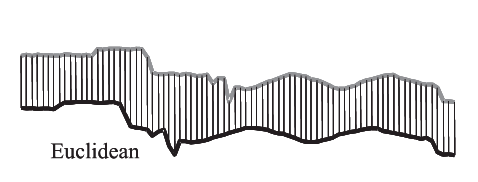
\includegraphics[width=0.5\columnwidth]{capitulos/imagens/distance.png}
        \caption{Representação da Distância Euclidiana}
	\end{center}
\end{figure}

Outras distâncias e relações entre elas podem ser vistas no livro de Deza e Deza~\citep{EncyclopediaofDistances}.

\section{Complexidade Estatística}

Por definição complexidade refere-se a um conjunto de coisas ligadas por um nexo comum. Inversamente à entropia, a complexidade estatística procura encontrar estruturas de interação e dependência entre os elementos de uma dada série, tratando-se de um fator extremamente importante no estudo de sistemas dinâmicos.

Essa propriedade é definida por meio da fórmula desenvolvida por Lopèz-Ruiz, Mancini e Calbet, onde uma Entropia e uma Distância, também chamada de desequilíbrio, podem ser combinadas no atributo Complexidade Estatística para aumentar o seu poder de descrição~\citep{article5,FELDMAN1998244,LOPEZRUIZ1995321}:

\begin{equation}
C(\bm h, \bm p) = H(\bm h)Q(\bm h, \bm p)
\end{equation}.

O desequilibrio $\bm Q$ reflete como se comporta a arquitetura do sistema analisado. Quando tal sistema possui alguma estrutura privilegiada ou estados mais prováveis entre os acessíveis, esse valor será diferente de zero.

Uma escolha conveniente é a complexidade de Jensen-Shannon, dada por

 \begin{equation}
 C_{\text{JS}}(\bm h) = H_{\text{S}}(\bm h) . Q_{\text{JS}}(\bm h, \bm p_e),
 \end{equation}
 
em que $H_{\text{S}}$ é a entropia de Shannon normalizada, $\bm h$ a função de probabilidade da série, $\bm p_e$ a distribuição uniforme e $Q_{\text{JS}}$ é a divergência de Jensen-Shannon, cuja importância da discutida em~\cite{LAMBERTI2004119}. Temos então:

\begin{equation}
Q(\bm h, \bm p_e) = Q_0 . J(\bm h, \bm p_e),
\end{equation}

Sendo,

\begin{equation}
J(\bm h, \bm p_e) = S\left(\frac{\bm h + \bm p_e}{2}\right) - \frac{S(\bm h)}{2} - \frac{S(\bm p_e)}{2},
\end{equation}

e $\bm Q_0$ uma constante de normalização, logo $0 \leq Q_0 \leq 1$, definida por:

\begin{equation}
Q_0 = -2 \left[ \left(\frac{N + 1}{N} \right) \ln(N + 1) - 2 \ln{2N} + \ln{N} \right]^{-1}.
\end{equation}

\section{Plano Complexidade-Entropia}

 O plano Complexidade-Entropia refere-se ao gráfico bidimensional entre a Entropia de Permutação Normalizada $H(p)$ (eixo horizontal) e a Complexidade Estatística $C(\bm p, \bm p_e)$ (eixo vertical). 

 Por intermédio de tal ferramenta é possível descobrir a natureza da série, determinando se esta corresponde a uma sequência caótica, estocástica ou determinística, analisando o seu comportamento, visto que estes possuem dinâmicas diferentes. De acordo com a segunda lei da termodinâmica:
 
 \begin{quote}
A quantidade de entropia de qualquer sistema isolado termodinamicamente tende a incrementar-se com o tempo, até alcançar um valor máximo. 
 \end{quote}

 Como a entropia varia uniformemente com o tempo, podemos concluir que o plano Complexidade-Entropia além de analisar a interação entre estas duas características, também verifica a evolução temporal de $C(\bm p, \bm p_e)$.

 O plano Entropia-Complexidade também é conhecido como “O plano de causalidade entre a entropia e a complexidade”, tendo em vista que no ramo da estatística causalidade refere-se a relação entre as causas dos fenômenos e seus respectivos efeitos e resultados. Assim, podemos inferir que como a própria nomenclatura sugere, o diagrama relaciona os dados resultantes do cálculo da entropia e da complexidade estatística e as suas características estimadas pela Teoria da Informação. 

\begin{figure}[!hbt]
	\begin{center}
		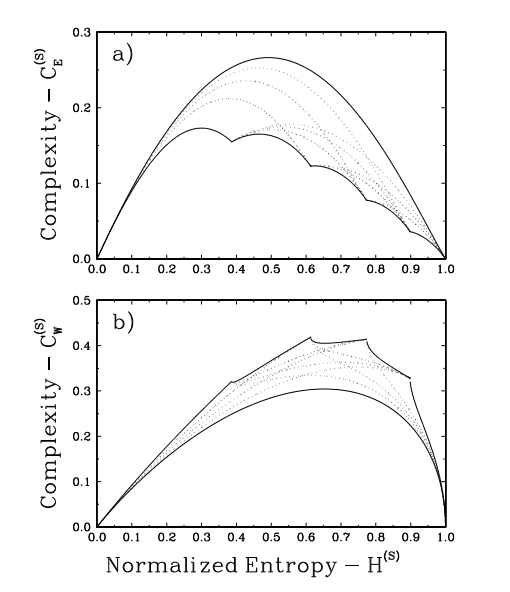
\includegraphics[width=0.6\columnwidth]{capitulos/imagens/graficoComplexidade.png}
        \caption{Gráficos Complexidade-Entropia em relação à entropia de Shannon e as distâncias Euclidiana e de Wootters.}
	\end{center}
\end{figure}
 
Cada série temporal $\bm X$ pode, então, ser mapeada no ponto $(H_{\text{S}}, C(\bm p, \bm p_e))$.
O conjunto de todos os pontos possíveis forma o \textit{mapa Entropia-Complexidade}, e a posição do ponto nesse plano é um descritor das propriedades da dinâmica subjacente à série~\citep{OrdinalPatternProbabilities}.
A forma desse plano depende do comprimento $D$ dos padrões~\citep{MARTIN2006439}.

\mychapter{Metodologia}{cap:metodologia}

A metodologia da pesquisa desenvolvida consistiu em dois grandes momentos, a etapa teórica e a implementação das funcionalidades.

Para o desenvolvimento do projeto descrito neste trabalho, foram planejadas as seguintes etapas de execução, que foram realizadas ao longo dos últimos meses.

\section{Estudo das funções a serem implementadas}

O estudo das funções a serem implementadas foi realizado a partir da análise de um conjunto de referências bibliográficas de qualidade, visando ampliar os conhecimentos a cerca do tema proposto.

Foram estudados ao longo deste momento, temas como séries temporais, suas propriedades e aplicações, Teoria da Informação, entropias~\cite{salicruetal1993}, distâncias estocásticas~\cite{StatisticalInferenceBasedonDivergenceMeasures}, complexidades estatísticas, plano HC e a linguagem de programação \texttt R.

\section{Implementação e validação numérica}

Após o término da revisão bibliográfica da literatura existente, foi dado então início à implementação do trabalho, desenvolvido em \texttt R e sempre fazendo uso de boas práticas de desenvolvimento de software científico.

Para que tal ferramenta seja aplicada na análise de dados é de suma importância realizar a verificação de suas propriedades numéricas. 
Portanto, a avaliação da qualidade numérica das funcionalidades desenvolvidas foi feita utilizando uma metodologia própria baseada em sistemas dinâmicos com saídas conhecidas.

\section{Análise de alternativas para o desenvolvimento da interface}

Um dos grandes objetivos da pesquisa consistia em ampliar a aplicabilidade das técnicas de extração de informações de séries temporais, por meio de uma ferramenta portável e interativa de análise. Assim, foram avaliadas algumas opções de ferramentas de GUI que fossem capaz de suportar as funcionalidades desenvolvidas em \texttt R na primeira etapa.

Foi então realizada uma pesquisa sobre as alternativas existentes sendo considerado os seguintes fatores:

\begin{itemize}
\item Portabilidade do software para os diversos sistemas operacionais e arquiteturas de hardware; 
\item Facilidade de instalação, pois uma vez que queremos por meio do desenvolvimento do projeto facilitar de um modo geral a análise de séries temporais na experiência do usuário, logo esta não deverá apresentar problemas no processo de instalação;
\item Integração com a linguagem de programação \texttt R.
\end{itemize}

Desse modo, \texttt{RGtk2} e \texttt{Java Swing} foram as alternativas iniciais para o desenvolvimento da interface gráfica. 
No entanto, após estudos sobre o funcionamento destas GUIs (\textit{Graphical User Interface}), verificamos que a implementação da interface utilizando \texttt{Java Swing} apresentava certos empecilhos em relação a portabilidade do software em diferentes sistemas operacionais, não satisfazendo ao item 1 de nossas exigências, seria necessário a implementação individual do software para cada sistema operacional, já que o programa deveria ser capaz de  reconhecer o sistema utilizado pelo cliente e assim executar seguindo as regras e padrões deste. Outro fator decisivo foram as dificuldades de comunicação entre o código \texttt{Java} e o script em \texttt{R}.

Portanto, optamos pelo \texttt{RGtk2}, por ser uma biblioteca própria do ambiente de desenvolvimento \texttt R e pela sua maior facilidade em manter a portabilidade do sistema.

\section{Desenvolvimento de protótipos}
 
Foram desenvolvidos alguns protótipos de modelos de interface com as alternativas de bibliotecas gráficas citadas anteriormente, sempre com foco na experiência do usuário. 

No entanto, por possuímos como objetivo o desenvolvimento de uma ferramenta \texttt{Desktop} algumas alterações foram realizadas para se adequar as funções oferecidas pela biblioteca escolhida.

\section{Versão de produção da interface}

Após a finalização do processo de escolha da biblioteca \texttt{RGtk2}, foi então dado início a implementação da interface.
Esta etapa consistiu basicamente da realizada da integração entre o ambiente gráfico do sistema e as funções de análise de séries temporais implementadas em fases anteriores.

\section{Validação, verificação e preparação de manuais e tutoriais de uso}

Como já citado, é de fundamental importância para tal projeto a verificação da qualidade numérica do software desenvolvido, portanto um dos seus objetivos consistiu em validar a interface e as funções com usuários finais.

Foram também desenvolvidos manuais de uso das funções implementadas, informando as suas funcionalidades, parâmetros de entrada e o resultado final computado. Todas essas descrições se encontram apresentados no apêndice A deste trabalho.

\mychapter{Resultados e Discussões}{cap:resultados}    

Apresentamos o desenvolvimento de uma ferramenta portável, rápida e de boa qualidade numérica que possibilita gerar novos métodos de interação do usuário com o sistema de análise, permitindo que este seja capaz de analisar os diferentes descritores oriundos da Teoria da Informação e permitir a análise gráfica dos resultados.

Seguindo o modelo de engenharia de software em espiral, o sistema foi projetado e desenvolvido de forma modular, composto pelas seguintes unidades:

\begin{itemize}
\item Módulo de simbolização;
\item Módulo de análise;
\item Modulo de visualização e interação (Em fase de desenvolvimento);
\end{itemize} 

Esses módulos foram e estão sendo desenvolvidos seguindo um cronograma. 
Depois passaram pelas seguintes etapas:

\begin{itemize}
\item Integração dos módulos em um sistema;
\item Teste e validação do sistema (em fase de desenvolvimento);
\item Geração da interface gráfica (em fase de desenvolvimento).
\end{itemize}

Permite-se a leitura de dados em vários formatos (TXT, CSV ou XLSX), e o usuário a seguir poderá escolher:

\begin{itemize}

	\item Gerar o gráfico da série (ver Figura 1);
	\item Calcular seus diversos valores de Entropia;
	\item Calcular seus diversos valores de Distâncias Estocásticas;
	\item Calcular complexidades estatísticas;
    \item Identificar padrões no gráfico da série temporal;
    \item Gerar planos de Entropias;
    \item Gerar planos de Distâncias Estocásticas;
	\item Gerar o histograma de padrões (ver Figura 1);
	\item Identificar o ponto característico da série no plano Entropia-Complexidade (ver Figura 1).

\end{itemize}

Um elemento original do sistema é a vinculação entre o histograma de padrões, formados através do processo de \textit{simbolização de}~\cite{article2}, e a série temporal. 
Escolhendo um ou mais elementos do histograma, os valores correspondentes na série temporal aparecem realçados. 
Esta funcionalidade permite a análise visual da distribuição temporal dos padrões, possibilitando futuramente a realização de outros testes.
 
O teste e a validação do sistema foram tarefas contínuas ao longo do desenvolvimento do projeto, bem como o incremento do desenvolvimento de novas funcionalidades. 

Com a troca da ferramenta de interface, foi necessário primeiramente um estudo de documentações referentes ao pacote gráfico~\cite{rgtk2}. 
Uma vez que ocorreu uma mudança de paradigmas pois a biblioteca escolhida funciona por meio de blocos verticais e horizontais, onde os horizontais se são distribuídos diante dos verticais, foram encontrados os seguintes problemas durante a implementação:

\begin{itemize}
\item A reprodução do modelo do protótipo;
\item A implementação da função referente a \texttt file.choose em \texttt R, pois o escopo das variáveis declaradas dentro das funções de tratamento de interrupções é local;
\item A implementação das funções de tratamento de interrupção;
\item O desenvolvimento da parte estética do software.
\end{itemize}

\begin{figure}
  \centering
  \caption{Imagem do protótipo do modelo desenvolvido}
   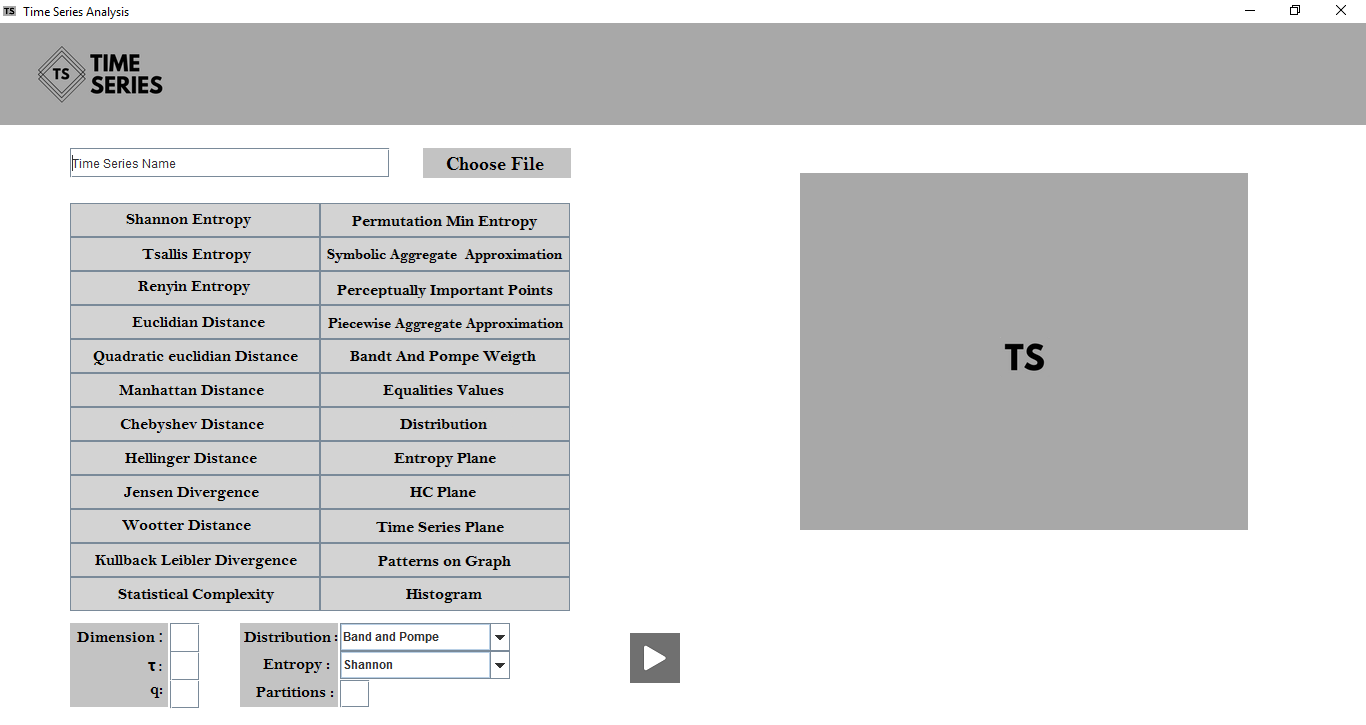
\includegraphics[width=15cm,height=7cm]{imagens/tela4.png}
\end{figure}

\begin{figure}
  \centering
  \caption{Estrutura de organização dos componentes no RGtk2}
   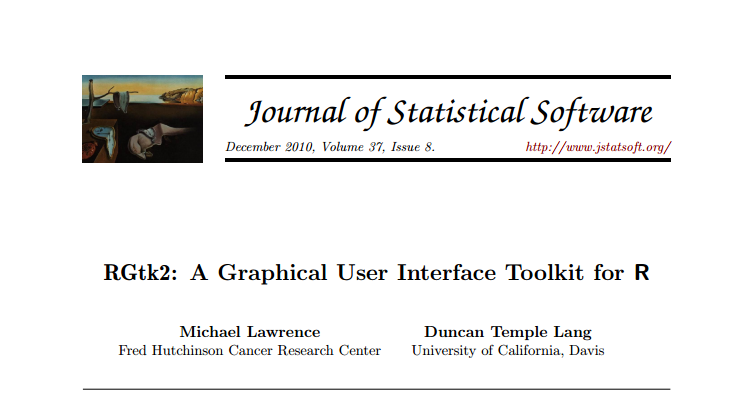
\includegraphics[width=10cm,height=6cm]{imagens/rgtk2.png}
\end{figure}
  
\begin{figure}[H]
	\centering
	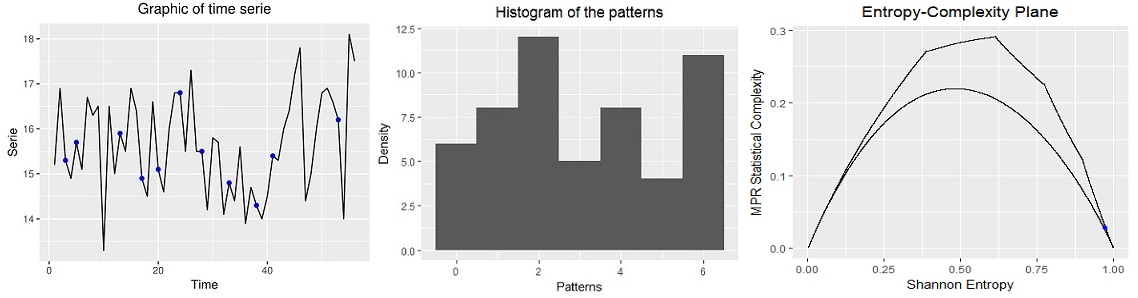
\includegraphics[width=1\columnwidth]{imagens/rplot}        
    \caption{Representação gráfica da análise de uma série temporal de produção anual de cevada por acre.}
\end{figure}
 
\begin{figure}[H]
	\centering
	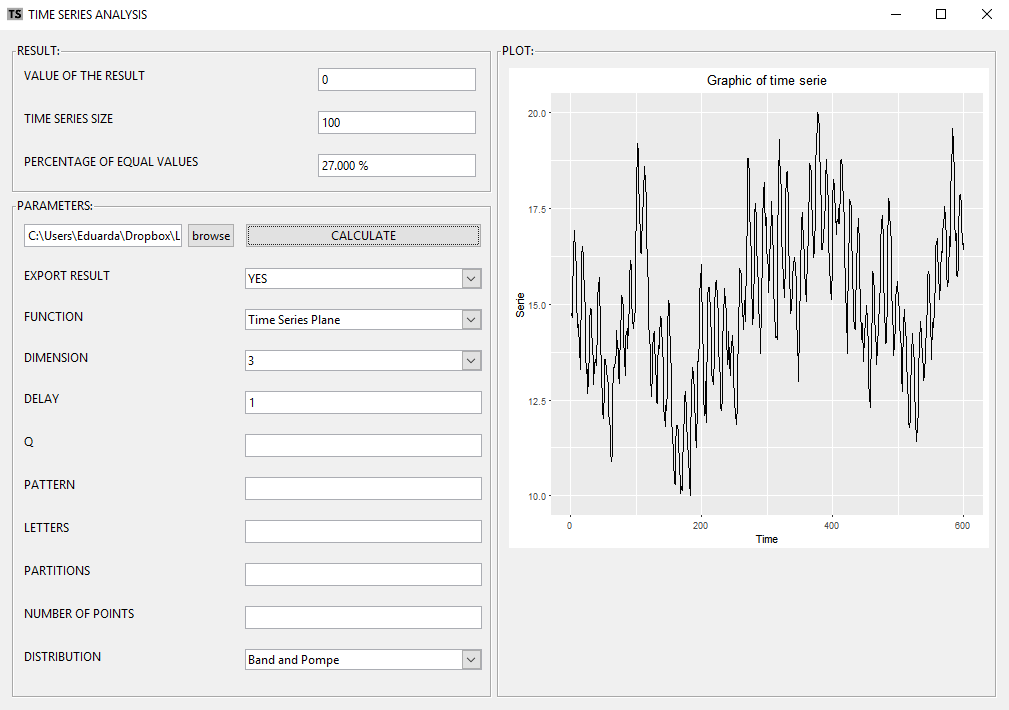
\includegraphics[width=0.95\columnwidth]{imagens/tms}   
    \caption{Imagem atual do software.}
    \vspace{6cm}
\end{figure}



\mychapter{Demonstração de uso do Software}{cap:demonstracao}

Nesta sessão, demonstraremos como utilizar a interface do Software desenvolvido para realizar a análise da caracterização do ruído colorido \footnote{\url{https://www.mathworks.com/matlabcentral/fileexchange/35381-noisefk-m}} de espectro de potência $f^{-3/2}$.

\section{Upload de dados} 

Primeiramente, iremos fazer upload do arquivo $.csv$ que contém os dados que serão utilizados. Para isso iremos clicar no botão \mybox{BROWSE} e selecionar o arquivo desejado (Figura~\ref{fig:Upload}).

\begin{figure}[H]
	\centering
	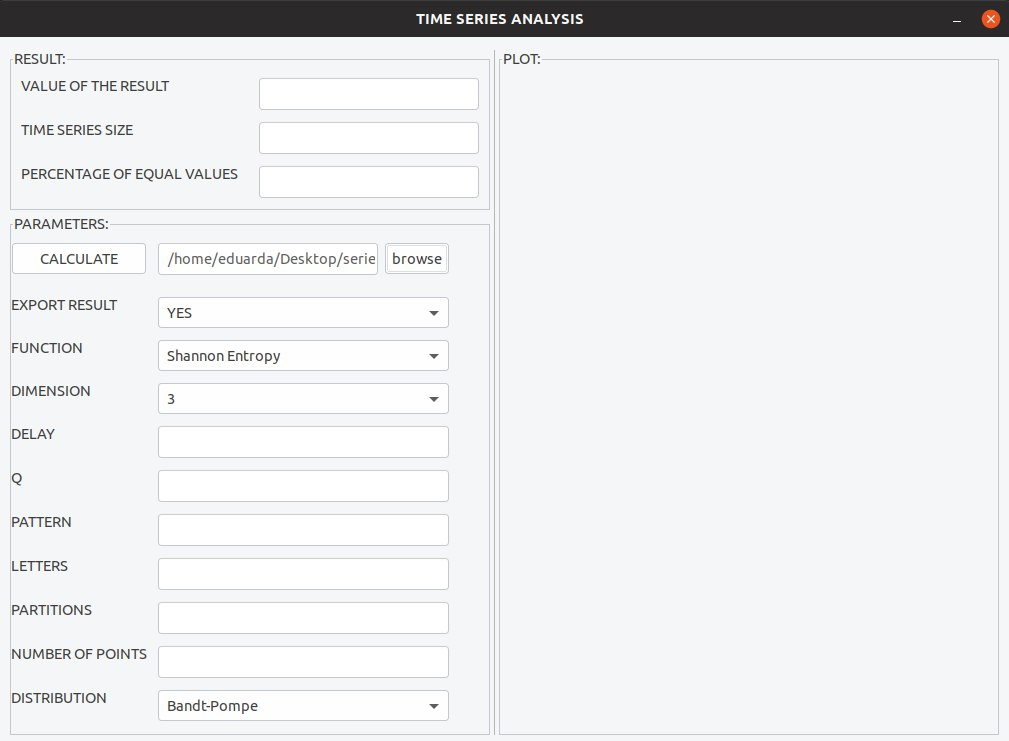
\includegraphics[width=0.85\columnwidth]{capitulos/imagens/Upload} 
    \caption{Upload do arquivo}
    \label{fig:Upload}
\end{figure}

\section{Visualização da série temporal}

O próximo passo será visualizar como se comporta a série temporal ao longo do tempo. Para isso, iremos selecionar dentro das possibilidades da variável \mybox{FUNCTION} a funcionalidade \mybox{Time Series Plane}.

Como podemos verificar, algumas informações básicas sobre os dados também são fornecidas, como o tamanho da série e o percentual de valores repetidos(Figura~\ref{fig:TimeSerie}).

O software também disponibiliza a opção de exportar os resultados obtidos em cada iteração com o usuário, para isso é necessário apenas habilitar a opção na variável \mybox{EXPORT RESULT}. Todos os devidos arquivos resultantes serão armazenados no mesmo diretório que o sistema se encontra.

\begin{figure}[H]
	\centering
	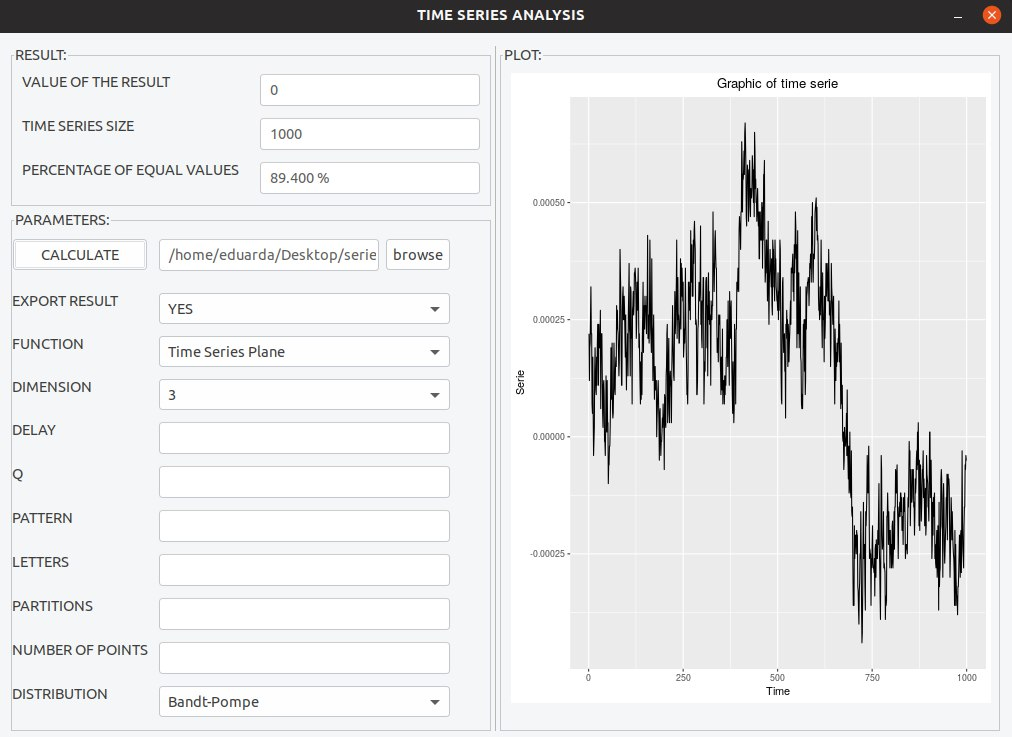
\includegraphics[width=0.85\columnwidth]{capitulos/imagens/timeSeriesPlot} 
    \caption{Gráfico do comportamento da Série Temporal}
    \label{fig:TimeSerie}
\end{figure}

\section{Histograma da distribuição de Bandt-Pompe} 

Assim como propõe a metodologia da simbolização, iremos agora visualizar como se comporta a distribuição dos padrões de Bandt-Pompe. Neste exemplo, aplicaremos valores de dimensão $D = 3$ e delay $\tau = 1$. Para isso, selecionaremos a funcionalidade \mybox{Histogram} e configuraremos a variável \mybox{DELAY} para o valor desejado (Figura~\ref{fig:bandtPompe}).

\begin{figure}[H]
	\centering
	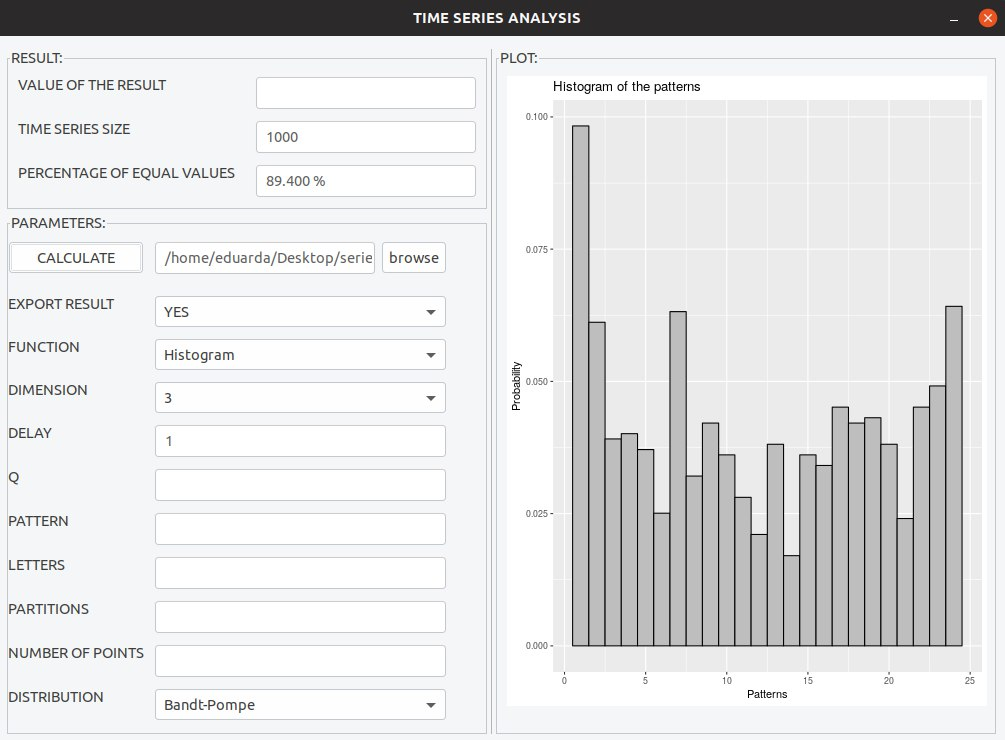
\includegraphics[width=0.85\columnwidth]{capitulos/imagens/Histogram} 
    \caption{Histograma da distribuição da probabilidade de Bandt-Pompe}
    \label{fig:bandtPompe}
\end{figure}

\section{Cálculo da Entropia de Shannon}

Para adquirir isoladamente o valor da Entropia de Permutação Normalizada de Shannon, devemos agora apenas selecionar a opção \mybox{Shannon Entropy} e pressionar o botão \mybox{CALCULATE} (Figura~\ref{fig:shannon}).

\begin{figure}[!hbt]
	\centering
	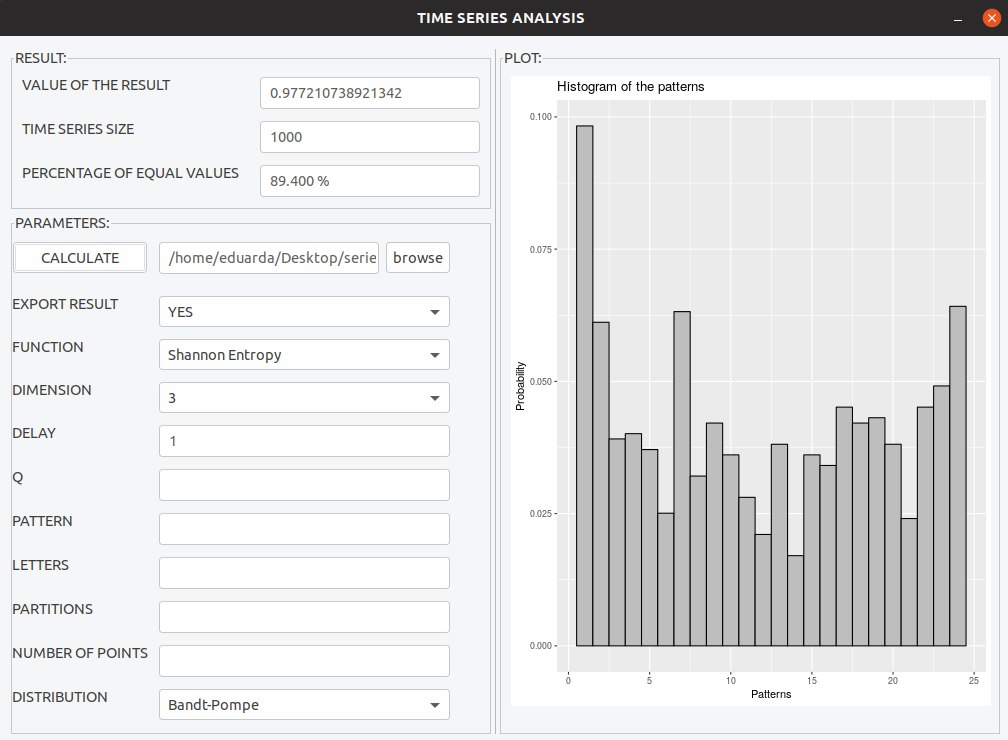
\includegraphics[width=0.85\columnwidth]{capitulos/imagens/Shannon} 
    \caption{Resultado obtido da Entropia de Shannon}
    \label{fig:shannon}
\end{figure}

\section{Cálculo da Complexidade Estatística}

De modo semelhante a Entropia, para possui o valor da Complexidade Estatística, devemos selecionar a opção \mybox{Statistical Complexity} e pressionar o botão \mybox{CALCULATE} (Figura~\ref{fig:complexity}).

\begin{figure}[!hbt]
	\centering
	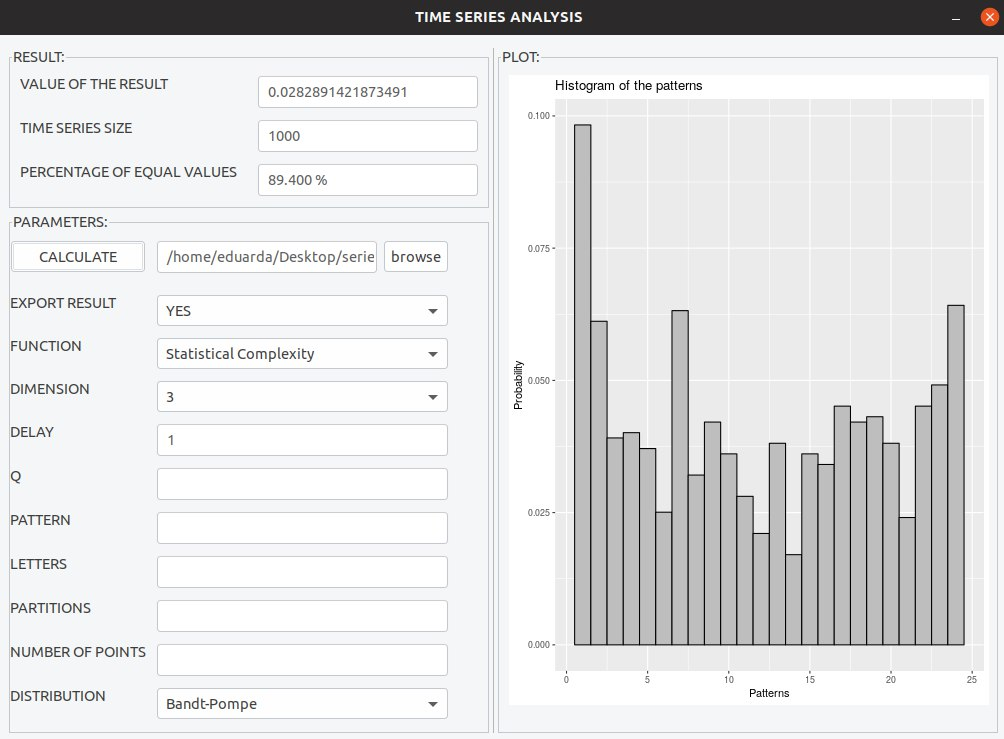
\includegraphics[width=0.85\columnwidth]{capitulos/imagens/complexity} 
    \caption{Resultado obtido da Complexidade Estatística}
    \label{fig:complexity}
\end{figure}

\section{Plano Complexidade-Entropia}

Por fim, uma vez que os valores referentes a dimensão $D$ e o delay $\tau$ já se encontram configurados, para gerar o Plano Complexidade-Entropia devemos apenas selecionar a opção \mybox{HC Plane} e informar em quantas partições queremos analisar a série, caso o valor informado seja superior a 1, a série irá ser dividida em subconjuntos e exibido os pontos correspondentes a cada um destes (Figura~\ref{fig:hCPlane}).

Como podemos observar, o comportamento descrito no plano corresponde ao valor já esperado na literatura~\citep{phdthesis}, o ruído $f^{-3/2}$ possui um alto valor de Entropia, ou seja alta desordem na estrutura da dinâmica dos seus dados e um baixo valor de Complexidade.

\begin{figure}[!hbt]
	\centering
	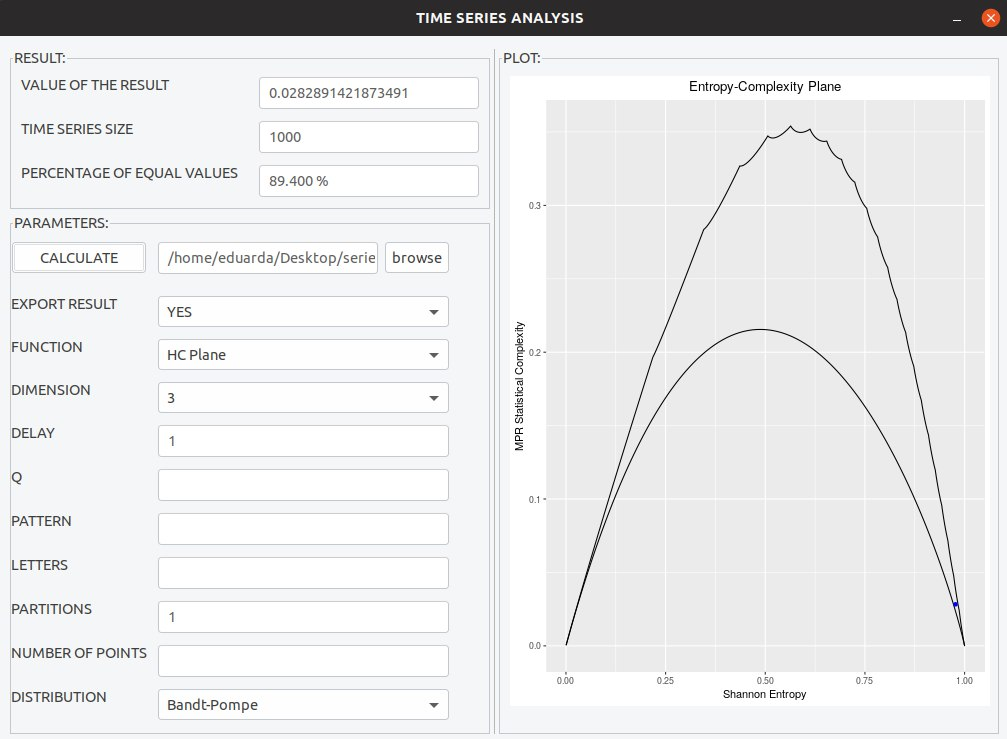
\includegraphics[width=0.85\columnwidth]{capitulos/imagens/hCPlane} 
    \caption{Caracterização do ruído $f^{-3/2}$ no Plano Complexidade-Entropia}
    \label{fig:hCPlane}
\end{figure}
\mychapter{Conclusões}{cap:conclusoes}

Neste capítulo serão abordados os avanços no meio científico e a importância proporcionada através do desenvolvimento deste trabalho. Além disso, também apresentaremos sugestões para futuros trabalhos.

\section{Considerações Finais}

Este trabalho propôs o desenvolvimento de uma ferramenta portável, rápida e de boa qualidade numérica que possibilita análises de uma série temporal através de descritores provenientes da Teoria da Informação. Para atribuir uma função de distribuição de probabilidade utilizamos o método de simbolização de Bandt-Pompe. A caracterização dos dados é dada por meio dos seus descritores, sendo então disponibilizadas diversas entropias, distâncias estocásticas e complexidade estatística.

Um elemento original do sistema é a vinculação entre o histograma de padrões e a série temporal. Escolhendo um ou mais elementos do histograma, os valores correspondentes na série temporal aparecem realçados. Esta funcionalidade permite a análise visual da distribuição temporal dos padrões, possibilitando futuramente a realização de outros testes.

O projeto também oferece aos pesquisadores a facilidade de utilização de técnicas sofisticadas da computação científica por meio de uma interface simples e intuitiva, sendo possível realizar em poucos passos atividades antes realizadas apenas por meio de scripts, exigindo assim mínimo conhecimento com programação por parte do usuário.

\section{Trabalhos futuros}

Pretendemos expandir as funcionalidades do sistema, dando agora ênfase ao problema da imputação de padrões ausentes. Para tanto, pretendemos atingir os seguintes objetivos:

\begin{itemize}
\item Estudar e implementar técnicas para imputação de padrões ausentes ocasionados por dados repetidos;
\item Analisar a capacidade de reconstrução de informações dessas técnicas quando a série temporal é armazenada com menos precisão do que a ideal;
\item Analisar a distribuição temporal dos padrões originais e imputados.
\end{itemize}

\selectlanguage{portuguese}
\appendix
\chapter{Manual de utilização das funções desenvolvidas} \label{apendiceA}

\section{Pacotes necessários}

Para que seja possível utilizar plenamente as funções desenvolvidas ao longo deste projeto será necessário que os seguintes pacotes estejam instalados no ambiente \textit{RStudio}:

\begin{itemize}
\item combinat
\item ggplot2
\item dygraphs
\item ggthemes
\end{itemize}

Após a instalação, o usuário pode realizar normalmente a chamadas das funções implementadas.

\section{Funções desenvolvidas}

%------------------------------------------------------------------------------------------------------------------

\hrulefill   

\begin{table}[!ht]
\begin{center}
\begin{tabularx}{\textwidth}{ X X}
\hspace{0.5cm} Readtxt & \textit{Leitura de dados de um arquivo .txt}\\
\end{tabularx}
\end{center}
\end{table} 

\vspace{-0.5cm}

\hrulefill  

\vspace{0.5cm}

\textbf{Uso}

\begin{lstlisting}
   Readtxt(column)
\end{lstlisting}

\vspace{0.5cm}

\textbf{Argumentos}

\begin{table}[!ht]
\begin{center}
\begin{tabularx}{\textwidth}{X X}
\hspace{0.5cm} \textit{column} & Coluna de dados que deseja ser lida pela função.\\
\end{tabularx}
\end{center}
\end{table} 

\newpage


%------------------------------------------------------------------------------------------------------------------

\hrulefill   

\begin{table}[!ht]
\begin{center}
\begin{tabularx}{\textwidth}{ X X}
\hspace{0.5cm} Readcsv & \textit{Leitura de dados de um arquivo .csv}\\
\end{tabularx}
\end{center}
\end{table} 

\vspace{-0.5cm}

\hrulefill  

\vspace{0.5cm}

\textbf{Uso}

\begin{lstlisting}
   Readcsv(column,separator)
\end{lstlisting}

\vspace{0.5cm}

\textbf{Argumentos}

\begin{table}[!ht]
\begin{center}
\begin{tabularx}{\textwidth}{X X}
\hspace{0.5cm} \textit{column} & Coluna de dados que deseja ser lida pela função.\\
\hspace{0.5cm} \textit{separator} & (Opcional) Caracter separador de campo. Os valores em cada linha do arquivo são separados por esse caracter. É colocado por default o ";".\\
\end{tabularx}
\end{center}
\end{table} 


%------------------------------------------------------------------------------------------------------------------

\hrulefill   

\begin{table}[!ht]
\begin{center}
\begin{tabularx}{\textwidth}{ X X}
\hspace{0.5cm} equalitiesValues & \textit{Percentual de dados repetidos em uma dada série temporal}\\
\end{tabularx}
\end{center}
\end{table} 

\vspace{-0.5cm}

\hrulefill  

\vspace{0.5cm}

\textbf{Uso}

\begin{lstlisting}
   equalitiesValues(serie)
\end{lstlisting}

\vspace{0.5cm}

\textbf{Argumentos}

\begin{table}[!ht]
\begin{center}
\begin{tabularx}{\textwidth}{X X}
\hspace{0.5cm} \textit{serie} & Um vetor numérico onde estará instânciada a série temporal que deve ser avaliada pela função.\\
\end{tabularx}
\end{center}
\end{table} 

\newpage

%------------------------------------------------------------------------------------------------------------------

\hrulefill   

\begin{table}[!ht]
\begin{center}
\begin{tabularx}{\textwidth}{X X}
\hspace{0.5cm} removeDuplicate & \textit{Remove os dados duplicados de uma série temporal}\\
\end{tabularx}
\end{center}
\end{table} 

\vspace{-0.5cm}

\hrulefill  

\vspace{0.5cm}

\textbf{Uso}

\begin{lstlisting}
   removeDuplicate(serie)
\end{lstlisting}

\vspace{0.5cm}

\textbf{Argumentos}

\begin{table}[!ht]
\begin{center}
\begin{tabularx}{\textwidth}{X X}
\hspace{0.5cm} \textit{serie} & Um vetor numérico onde estará instânciada a série temporal que deve ser avaliada pela função.\\
\end{tabularx}
\end{center}
\end{table} 

%------------------------------------------------------------------------------------------------------------------

\hrulefill   

\begin{table}[!ht]
\begin{center}
\begin{tabularx}{\textwidth}{X X}
\hspace{0.5cm} distribution & \textit{Distribuição de probabilidade de Bandt and Pompe}\\
\end{tabularx}
\end{center}
\end{table} 

\vspace{-0.5cm}

\hrulefill  

\vspace{0.5cm}

\textbf{Uso}

\begin{lstlisting}
   distribution(serie,dimension,delay)
\end{lstlisting}

\vspace{0.5cm}

\textbf{Argumentos}

\begin{table}[!ht]
\begin{center}
\begin{tabularx}{\textwidth}{X X}
\hspace{0.5cm} \textit{serie} \vspace{0.5cm}& Um vetor numérico onde estará instânciada a série temporal que deve ser avaliada pela função.\vspace{0.5cm}\\
\hspace{0.5cm} \textit{dimension} \vspace{0.5cm}& Dimensão dos padrões ordinais.\vspace{0.5cm}\\
\hspace{0.5cm} \textit{delay} & Delay utilizado na formação dos padrões.\\
\end{tabularx}
\end{center}
\end{table} 

\newpage

%------------------------------------------------------------------------------------------------------------------

\hrulefill   

\begin{table}[!ht]
\begin{center}
\begin{tabularx}{\textwidth}{X X}
\hspace{0.5cm} WPE & Distribuição de probabilidade de Bandt and Pompe Weigth.\\
\end{tabularx}
\end{center}
\end{table} 

\vspace{-0.5cm}

\hrulefill  

\vspace{0.5cm}

\textbf{Uso}

\begin{lstlisting}
   WPE(serie,dimension,delay)
\end{lstlisting}

\vspace{0.5cm}


\textbf{Argumentos}

\begin{table}[!ht]
\begin{center}
\begin{tabularx}{\textwidth}{X X}
\hspace{0.5cm} \textit{serie} \vspace{0.5cm}& Um vetor numérico onde estará instânciada a série temporal que deve ser avaliada pela função.\vspace{0.5cm}\\
\hspace{0.5cm} \textit{dimension} \vspace{0.5cm}& Dimensão dos padrões ordinais.\vspace{0.5cm}\\
\hspace{0.5cm} \textit{delay} & Delay utilizado na formação dos padrões.\\
\end{tabularx}
\end{center}
\end{table} 

%---------------------------------------------------------------------------------------------------------------

\hrulefill   

\begin{table}[!ht]
\begin{center}
\begin{tabularx}{\textwidth}{ X X}
  \hspace{0.5cm} shannonEntropy & \textit{Entropia de Shannon de uma dada distribuição de probabilidade}\\
\end{tabularx}
\end{center}
\end{table} 

\vspace{-0.5cm}

\hrulefill  

\vspace{0.5cm}

\textbf{Uso}

\begin{lstlisting}
   shannonEntropy(p)
\end{lstlisting}

\vspace{0.5cm}

\textbf{Argumentos}

\begin{table}[!ht]
\begin{center}
\begin{tabularx}{\textwidth}{X X}
\hspace{0.5cm} \textit{p} & Uma distribuição de padrão ordinal.\\
\end{tabularx}
\end{center}
\end{table} 

\newpage
%---------------------------------------------------------------------------------------------------------------

\hrulefill   

\begin{table}[!ht]
\begin{center}
\begin{tabularx}{\textwidth}{ X X}
\hspace{0.5cm} shannonNormalized & \textit{Entropia normalizada de Shannon de uma distribuição de probabilidade}\\
\end{tabularx}
\end{center}
\end{table} 

\vspace{-0.5cm}

\hrulefill  

\vspace{0.5cm}

\textbf{Uso}

\begin{lstlisting}
   shannonNormalized(p)
\end{lstlisting}

\vspace{0.5cm}

\textbf{Argumentos}

\begin{table}[!ht]
\begin{center}
\begin{tabularx}{\textwidth}{X X}
\hspace{0.5cm} \textit{p} & Uma distribuição de padrão ordinal.\\
\end{tabularx}
\end{center}
\end{table} 

%---------------------------------------------------------------------------------------------------------------
\hrulefill   

\begin{table}[!ht]
\begin{center}
\begin{tabularx}{\textwidth}{ X X}
\hspace{0.5cm} tsallisEntropy & \textit{Entropia de Tsallis de uma dada distribuição de probabilidade}\\
\end{tabularx}
\end{center}
\end{table} 

\vspace{-0.5cm}

\hrulefill  

\vspace{0.5cm}

\textbf{Uso}

\begin{lstlisting}
   tsallisEntropy(p,q)
\end{lstlisting}

\vspace{0.5cm}

\textbf{Argumentos}

\begin{table}[!ht]
\begin{center}
\begin{tabularx}{\textwidth}{X X}
\hspace{0.5cm} \textit{p} \vspace{0.5cm}& Uma distribuição de padrão ordinal.\vspace{0.5cm}\\
\hspace{0.5cm} \textit{q} \vspace{0.5cm}& A ordem da entropia. Permite apenas números positivos.\vspace{0.5cm}\\
\end{tabularx}
\end{center}
\end{table} 

\newpage
%---------------------------------------------------------------------------------------------------------------

\hrulefill   

\begin{table}[!ht]
\begin{center}
\begin{tabularx}{\textwidth}{ X X}
\hspace{0.5cm} tsallisNormalized & \textit{Entropia normalizada de Tsallis de uma distribuição de probabilidade}\\
\end{tabularx}
\end{center}
\end{table} 

\vspace{-0.5cm}

\hrulefill  

\vspace{0.5cm}

\textbf{Uso}

\begin{lstlisting}
   tsallisNormalized(p,q)
\end{lstlisting}

\vspace{0.5cm}

\textbf{Argumentos}

\begin{table}[!ht]
\begin{center}
\begin{tabularx}{\textwidth}{X X}
\hspace{0.5cm} \textit{p} \vspace{0.5cm}& Uma distribuição de padrão ordinal.\vspace{0.5cm}\\
\hspace{0.5cm} \textit{q} \vspace{0.5cm}&  A ordem da entropia. Permite apenas números positivos.\vspace{0.5cm}\\
\end{tabularx}
\end{center}
\end{table} 

%---------------------------------------------------------------------------------------------------------------

\hrulefill   

\begin{table}[!ht]
\begin{center}
\begin{tabularx}{\textwidth}{ X X}
\hspace{0.5cm} renyiEntropy & \textit{Entropia de Renyi de uma distribuição de probabilidade}\\
\end{tabularx}
\end{center}
\end{table} 

\vspace{-0.5cm}

\hrulefill  

\vspace{0.5cm}

\textbf{Uso}

\begin{lstlisting}
   renyiEntropy(p,q)
\end{lstlisting}

\vspace{0.5cm}

\textbf{Argumentos}

\begin{table}[!ht]
\begin{center}
\begin{tabularx}{\textwidth}{X X}
\hspace{0.5cm} \textit{p} \vspace{0.5cm}& Uma distribuição de padrão ordinal.\vspace{0.5cm}\\
\hspace{0.5cm} \textit{q} \vspace{0.5cm}& A ordem da entropia. Permite apenas números positivos.\vspace{0.5cm}\\
\end{tabularx}
\end{center}
\end{table} 
\newpage

%---------------------------------------------------------------------------------------------------------------

\hrulefill   

\begin{table}[!ht]
\begin{center}
\begin{tabularx}{\textwidth}{ X X}
\hspace{0.5cm} renyiNormalized & \textit{Entropia normalizada de Renyi de uma distribuição de probabilidade}\\
\end{tabularx}
\end{center}
\end{table} 

\vspace{-0.5cm}

\hrulefill  

\vspace{0.5cm}

\textbf{Uso}

\begin{lstlisting}
   renyiNormalized(p,q)
\end{lstlisting}

\vspace{0.5cm}

\textbf{Argumentos}

\begin{table}[!ht]
\begin{center}
\begin{tabularx}{\textwidth}{X X}
\hspace{0.5cm} \textit{p} \vspace{0.5cm}& Uma distribuição de padrão ordinal.\vspace{0.5cm}\\
\hspace{0.5cm} \textit{q} \vspace{0.5cm}& A ordem da entropia. Permite apenas números positivos.\vspace{0.5cm}\\
\end{tabularx}
\end{center}
\end{table} 

%---------------------------------------------------------------------------------------------------------------

\hrulefill   

\begin{table}[!ht]
\begin{center}
\begin{tabularx}{\textwidth}{ X X}
\hspace{0.5cm} PME & \textit{Entropia entropia de mínima permutação de uma distribuição de probabilidade}\\
\end{tabularx}
\end{center}
\end{table} 

\vspace{-0.5cm}

\hrulefill  

\vspace{0.5cm}

\textbf{Uso}

\begin{lstlisting}
   PME(p)
\end{lstlisting}

\vspace{0.5cm}

\textbf{Argumentos}

\begin{table}[!ht]
\begin{center}
\begin{tabularx}{\textwidth}{X X}
\hspace{0.5cm} \textit{p} & Uma distribuição de padrão ordinal.\\
\end{tabularx}
\end{center}
\end{table} 
\newpage
%------------------------------------------------------------------------------------------------------

\hrulefill   

\begin{table}[!ht]
\begin{center}
\begin{tabularx}{\textwidth}{ X X}
\hspace{0.5cm} euclidianDistance & \textit{Distância euclidiana de uma dada distribuição de probabilidade e a distribuição de probabilidade uniforme}\\
\end{tabularx}
\end{center}
\end{table} 

\vspace{-0.5cm}

\hrulefill  

\vspace{0.5cm}

\textbf{Uso}

\begin{lstlisting}
   euclidianDistance(p)
\end{lstlisting}

\vspace{0.5cm}

\textbf{Argumentos}

\begin{table}[!ht]
\begin{center}
\begin{tabularx}{\textwidth}{X X}
\hspace{0.5cm} \textit{p} & Uma distribuição de padrão ordinal.\\
\end{tabularx}
\end{center}
\end{table} 

%---------------------------------------------------------------------------------------------------------------

\hrulefill   

\begin{table}[!ht]
\begin{center}
\begin{tabularx}{\textwidth}{ X X}
\hspace{0.5cm} squaredDistance & \textit{Distância euclidiana quadrada de uma dada distribuição de probabilidade e a distribuição de probabilidade uniforme}\\
\end{tabularx}
\end{center}
\end{table} 

\vspace{-0.5cm}

\hrulefill  

\vspace{0.5cm}

\textbf{Uso}

\begin{lstlisting}
   squaredDistance(p)
\end{lstlisting}

\vspace{0.5cm}

\textbf{Argumentos}

\begin{table}[!ht]
\begin{center}
\begin{tabularx}{\textwidth}{X X}
\hspace{0.5cm} \textit{p} & Uma distribuição de padrão ordinal.\\
\end{tabularx}
\end{center}
\end{table} 

\newpage

%---------------------------------------------------------------------------------------------------------------

\hrulefill   

\begin{table}[!ht]
\begin{center}
\begin{tabularx}{\textwidth}{ X X}
\hspace{0.5cm} manhattanDistance & \textit{Distância de Manhattan de uma dada distribuição de probabilidade e a distribuição de probabilidade uniforme}\\
\end{tabularx}
\end{center}
\end{table} 

\vspace{-0.5cm}

\hrulefill  

\vspace{0.5cm}

\textbf{Uso}

\begin{lstlisting}
   manhattanDistance(p)
\end{lstlisting}

\vspace{0.5cm}

\textbf{Argumentos}

\begin{table}[!ht]
\begin{center}
\begin{tabularx}{\textwidth}{X X}
\hspace{0.5cm} \textit{p} & Uma distribuição de padrão ordinal.\\
\end{tabularx}
\end{center}
\end{table} 
%---------------------------------------------------------------------------------------------------------------

\hrulefill   

\begin{table}[!ht]
\begin{center}
\begin{tabularx}{\textwidth}{ X X}
\hspace{0.5cm} chebyshevDistance & \textit{Distância de Chebyshev de uma dada distribuição de probabilidade e a distribuição de probabilidade uniforme}\\
\end{tabularx}
\end{center}
\end{table} 

\vspace{-0.5cm}

\hrulefill  

\vspace{0.5cm}

\textbf{Uso}

\begin{lstlisting}
   chebyshevDistance(p)
\end{lstlisting}

\vspace{0.5cm}

\textbf{Argumentos}

\begin{table}[!ht]
\begin{center}
\begin{tabularx}{\textwidth}{X X}
\hspace{0.5cm} \textit{p} & Uma distribuição de padrão ordinal.\\
\end{tabularx}
\end{center}
\end{table} 

\newpage

%---------------------------------------------------------------------------------------------------------------

\hrulefill   

\begin{table}[!ht]
\begin{center}
\begin{tabularx}{\textwidth}{ X X}
\hspace{0.5cm} hellingerDistance & \textit{Distância  de Hellinger de uma dada distribuição de probabilidade e a distribuição de probabilidade uniforme}\\
\end{tabularx}
\end{center}
\end{table} 

\vspace{-0.5cm}

\hrulefill  

\vspace{0.5cm}

\textbf{Uso}

\begin{lstlisting}
   hellingerDistance(p)
\end{lstlisting}

\vspace{0.5cm}

\textbf{Argumentos}

\begin{table}[!ht]
\begin{center}
\begin{tabularx}{\textwidth}{X X}
\hspace{0.5cm} \textit{p} & Uma distribuição de padrão ordinal.\\
\end{tabularx}
\end{center}
\end{table} 

%---------------------------------------------------------------------------------------------------------------

\hrulefill   

\begin{table}[!ht]
\begin{center}
\begin{tabularx}{\textwidth}{ X X}
\hspace{0.5cm} jensenDivergence & \textit{Medida de desequilíbrio generalizado para distribuições de probabilidade com base na divergência de Jensen-Shannon}\\
\end{tabularx}
\end{center}
\end{table} 

\vspace{-0.5cm}

\hrulefill  

\vspace{0.5cm}

\textbf{Uso}

\begin{lstlisting}
   jensenDivergence(p)
\end{lstlisting}

\vspace{0.5cm}

\textbf{Argumentos}

\begin{table}[!ht]
\begin{center}
\begin{tabularx}{\textwidth}{X X}
\hspace{0.5cm} \textit{p} & Uma distribuição de padrão ordinal.\\
\end{tabularx}
\end{center}
\end{table} 

\newpage
%---------------------------------------------------------------------------------------------------------------

\hrulefill   

\begin{table}[!ht]
\begin{center}
\begin{tabularx}{\textwidth}{ X X}
\hspace{0.5cm} woottersDistance & \textit{Distância de Wootters de uma dada distribuição de probabilidade e a distribuição de probabilidade uniforme}\\
\end{tabularx}
\end{center}
\end{table} 

\vspace{-0.5cm}

\hrulefill  

\vspace{0.5cm}

\textbf{Uso}

\begin{lstlisting}
   woottersDistance(p)
\end{lstlisting}

\vspace{0.5cm}

\textbf{Argumentos}

\begin{table}[!ht]
\begin{center}
\begin{tabularx}{\textwidth}{X X}
\hspace{0.5cm} \textit{p} & Uma distribuição de padrão ordinal.\\
\end{tabularx}
\end{center}
\end{table} 
%---------------------------------------------------------------------------------------------------------------

\hrulefill   

\begin{table}[!ht]
\begin{center}
\begin{tabularx}{\textwidth}{ X X}
\hspace{0.5cm} kullbackDivergence & \textit{Medida de desequilíbrio generalizado para distribuições de probabilidade com base na divergência de kullback-Leibler}\\
\end{tabularx}
\end{center}
\end{table} 

\vspace{-0.5cm}

\hrulefill  

\vspace{0.5cm}

\textbf{Uso}

\begin{lstlisting}
   kullbackDivergence(p)
\end{lstlisting}

\vspace{0.5cm}

\textbf{Argumentos}

\begin{table}[!ht]
\begin{center}
\begin{tabularx}{\textwidth}{X X}
\hspace{0.5cm} \textit{p} & Uma distribuição de padrão ordinal.\\
\end{tabularx}
\end{center}
\end{table} 

\newpage

%---------------------------------------------------------------------------------------------------------------

\hrulefill   

\begin{table}[!ht]
\begin{center}
\begin{tabularx}{\textwidth}{ X X}
\hspace{0.5cm} bhattacharyyaDistance & \textit{Distância de Bhattacharyya de uma dada distribuição de probabilidade e a distribuição de probabilidade uniforme}\\
\end{tabularx}
\end{center}
\end{table} 

\vspace{-0.5cm}

\hrulefill  

\vspace{0.5cm}

\textbf{Uso}

\begin{lstlisting}
   bhattacharyyaDistance(p)
\end{lstlisting}

\vspace{0.5cm}

\textbf{Argumentos}

\begin{table}[!ht]
\begin{center}
\begin{tabularx}{\textwidth}{X X}
\hspace{0.5cm} \textit{p} & Uma distribuição de padrão ordinal.\\
\end{tabularx}
\end{center}
\end{table} 
%----------------------------------------------------------------------------------------------------------

\hrulefill   

\begin{table}[!ht]
\begin{center}
\begin{tabularx}{\textwidth}{ X X}
\hspace{0.5cm} Ccomplexity & \textit{Complexidade estatística de uma distribuição de probabilidade}\\
\end{tabularx}
\end{center}
\end{table} 

\vspace{-0.5cm}

\hrulefill  

\vspace{0.5cm}

\textbf{Uso}

\begin{lstlisting}
   Ccomplexity(p)
\end{lstlisting}

\vspace{0.5cm}

\textbf{Argumentos}

\begin{table}[!ht]
\begin{center}
\begin{tabularx}{\textwidth}{X X}
\hspace{0.5cm} \textit{p} & Uma distribuição de padrão ordinal.\\
\end{tabularx}
\end{center}
\end{table} 

\newpage
%----------------------------------------------------------------------------------------------------------

\hrulefill   

\begin{table}[!ht]
\begin{center}
\begin{tabularx}{\textwidth}{ X X}
\hspace{0.5cm} timeSeries & \textit{Gráfico da série temporal}\\
\end{tabularx}
\end{center}
\end{table} 

\vspace{-0.5cm}

\hrulefill  

\vspace{0.5cm}

\textbf{Uso}

\begin{lstlisting}
   timeSeries(serie)
\end{lstlisting}

\vspace{0.5cm}

\textbf{Argumentos}

\begin{table}[!ht]
\begin{center}
\begin{tabularx}{\textwidth}{X X}
\hspace{0.5cm} \textit{serie} & Um vetor numérico onde estará instânciada a série temporal que deve ser avaliada pela função.\\
\end{tabularx}
\end{center}
\end{table} 
%---------------------------------------------------------------------------------------------------------------

\hrulefill   

\begin{table}[!ht]
\begin{center}
\begin{tabularx}{\textwidth}{ X X}
\hspace{0.5cm} histogram & \textit{Histograma dos padrões de Bandt and Pompe de uma série temporal}\\
\end{tabularx}
\end{center}
\end{table} 

\vspace{-0.5cm}

\hrulefill  

\vspace{0.5cm}

\textbf{Uso}

\begin{lstlisting}
   histogram(serie,dimension,delay)
\end{lstlisting}

\vspace{0.5cm}

\textbf{Argumentos}

\begin{table}[!ht]
\begin{center}
\begin{tabularx}{\textwidth}{X X}
\hspace{0.5cm} \textit{serie} \vspace{0.5cm}& Um vetor numérico onde estará instânciada a série temporal que deve ser avaliada pela função.\vspace{0.5cm}\\
\hspace{0.5cm} \textit{dimension} \vspace{0.5cm}& Dimensão dos padrões ordinais.\vspace{0.5cm}\\
\hspace{0.5cm} \textit{delay} \vspace{0.5cm}& Delay utilizado na formação dos padrões.\vspace{0.5cm}\\
\end{tabularx}
\end{center}
\end{table} 

\newpage
%---------------------------------------------------------------------------------------------------------------

\hrulefill   

\begin{table}[!ht]
\begin{center}
\begin{tabularx}{\textwidth}{ X X}
\hspace{0.5cm} patternsOnGraph & \textit{Localiza os pontos de uma série temporal pertencentes a um certo padrão ordinal}
\end{tabularx}
\end{center}
\end{table} 

\vspace{-0.5cm}

\hrulefill  

\vspace{0.5cm}

\textbf{Uso}

\begin{lstlisting}
   patternsOnGraph(serie,dimension,delay,pattern)
\end{lstlisting}

\vspace{0.5cm}

\textbf{Argumentos}

\begin{table}[!ht]
\begin{center}
\begin{tabularx}{\textwidth}{X X}
\hspace{0.5cm} \textit{serie} \vspace{0.5cm}& Um vetor numérico onde estará instânciada a série temporal que deve ser avaliada pela função.\vspace{0.5cm}\\
\hspace{0.5cm} \textit{dimension} \vspace{0.5cm}& Dimensão dos padrões ordinais.\vspace{0.5cm}\\
\hspace{0.5cm} \textit{delay} \vspace{0.5cm}& Delay utilizado na formação dos padrões.\vspace{0.5cm}\\
\hspace{0.5cm} \textit{pattern} \vspace{0.5cm}& Padrão que deverá ser analisado. Valor baseado nos padrões demonstrados no histograma.\vspace{0.5cm}\\
\end{tabularx}
\end{center}
\end{table} 
\newpage
%---------------------------------------------------------------------------------------------------------------

\hrulefill   

\begin{table}[!ht]
\begin{center}
\begin{tabularx}{\textwidth}{ X X}
\hspace{0.5cm} entropyPlane & \textit{Plota o gráfico da entropia de uma certa série temporal ou seus particionamentos}\\
\end{tabularx}
\end{center}
\end{table} 

\vspace{-0.5cm}

\hrulefill  

\vspace{0.5cm}

\textbf{Uso}

\begin{lstlisting}
   entropyPlane(serie,partitions,dimension,delay,
   			distribution,option,q)
\end{lstlisting}

\vspace{0.5cm}

\textbf{Argumentos}

\begin{table}[!ht]
\begin{center}
\begin{tabularx}{\textwidth}{X X}
\hspace{0.5cm} \textit{serie} \vspace{0.5cm}& Um vetor numérico onde estará instânciada a série temporal que deve ser avaliada pela função.\vspace{0.5cm}\\
\hspace{0.5cm} \textit{partitions} \vspace{0.5cm}& Quantidade de partições que a série deve ser dividida para a análise.\vspace{0.5cm}\\
\hspace{0.5cm} \textit{dimension} \vspace{0.5cm}& Dimensão dos padrões ordinais.\vspace{0.5cm}\\
\hspace{0.5cm} \textit{delay} \vspace{0.5cm}& Delay utilizado na formação dos padrões.\vspace{0.5cm}\\
\hspace{0.5cm} \textit{distribution} \vspace{0.5cm}& Distribuição que deve ser utilizada. O parâmetro deverá ser 1 para a distribuição de Bandt and Pompe, caso contrário a distribuição que será aplicada será a de Bandt and Pompe weigth.\vspace{0.5cm}\\
\hspace{0.5cm} \textit{option} \vspace{0.5cm}& Entropia que deve ser analisada. O parâmetro deve ser 1 para a entropia de shannon, 2 para a entropia de Tsallis ou 3 para a entropia de Renyi. Caso contrário, deverá ser aplicada a min entropy.\vspace{0.5cm}\\
\hspace{0.5cm} \textit{q} \vspace{0.5cm}& (Pode não ser necessário dependendo da entropia selecionada) Ordem da entropia.\vspace{0.5cm}\\
\end{tabularx}
\end{center}
\end{table} 

\newpage
%---------------------------------------------------------------------------------------------------------------

\hrulefill   

\begin{table}[!ht]
\begin{center}
\begin{tabularx}{\textwidth}{ X X}
\hspace{0.5cm} distancePlane & \textit{Plota o gráfico da distância estocástica de uma certa série temporal ou seus particionamentos}\\
\end{tabularx}
\end{center}
\end{table} 

\vspace{-0.5cm}

\hrulefill  

\vspace{0.5cm}

\textbf{Uso}

\begin{lstlisting}
   distancePlane<-function(serie,partition,dimension,delay,
   				optionD=1,optionP=1,q=1){
\end{lstlisting}

\vspace{0.5cm}

\textbf{Argumentos}

\begin{table}[!ht]
\begin{center}
\begin{tabularx}{\textwidth}{X X}
\hspace{0.5cm} \textit{serie} \vspace{0.5cm}& Um vetor numérico onde estará instânciada a série temporal que deve ser avaliada pela função.\vspace{0.5cm}\\
\hspace{0.5cm} \textit{partition} \vspace{0.5cm}& Quantidade de partições que a série deve ser dividida para a análise.\vspace{0.5cm}\\
\hspace{0.5cm} \textit{dimension} \vspace{0.5cm}& Dimensão dos padrões ordinais.\vspace{0.5cm}\\
\hspace{0.5cm} \textit{delay} \vspace{0.5cm}& Delay utilizado na formação dos padrões.\vspace{0.5cm}\\
\hspace{0.5cm} \textit{optionD} \vspace{0.5cm}& Distância estocástica que deve ser analisada. Devem ser usados os seguintes valores para acessar as opções disponíveis: Euclidiana (1), euclidiana quadrática (2), manhattan (3), chebyshev (4), divergência de Kullback-Leibler (5), helinger (6), divergência de Jensen Shannon (7), wootters (8) e bhattacharyya (9)\vspace{0.5cm}\\
\hspace{0.5cm} \textit{optionP} \vspace{0.5cm}& Distribuição que deve ser utilizada. O parâmetro deverá ser 1 para a distribuição de Bandt and Pompe, caso contrário a distribuição que será aplicada será a de Bandt and Pompe weigth.\vspace{0.5cm}\\
\end{tabularx}
\end{center}
\end{table} 

\begin{table}[!ht]
\begin{center}
\begin{tabularx}{\textwidth}{X X}
\hspace{0.5cm} \textit{q} \vspace{0.5cm}& (Pode não ser necessário dependendo da entropia selecionada) Ordem da entropia.\vspace{0.5cm}\\
\end{tabularx}
\end{center}
\end{table} 

\newpage

%---------------------------------------------------------------------------------------------------------------

\hrulefill   

\begin{table}[!ht]
\begin{center}
\begin{tabularx}{\textwidth}{ X X}
\hspace{0.5cm} partitionMPR & \textit{Gráfico entropia complexidade de uma série temporal ou de seus particionamentos}\\
\end{tabularx}
\end{center}
\end{table} 

\vspace{-0.5cm}

\hrulefill  

\vspace{0.5cm}

\textbf{Uso}

\begin{lstlisting}
   partitionMPR(serie,dimension,delay,partitions)
\end{lstlisting}

\vspace{0.5cm}

\textbf{Argumentos}

\begin{table}[!ht]
\begin{center}
\begin{tabularx}{\textwidth}{X X}
\hspace{0.5cm} \textit{serie} \vspace{0.5cm}& Um vetor numérico onde estará instânciada a série temporal que deve ser avaliada pela função.\vspace{0.5cm}\\
\hspace{0.5cm} \textit{dimension} \vspace{0.5cm}& Dimensão dos padrões ordinais.\vspace{0.5cm}\\
\hspace{0.5cm} \textit{delay} \vspace{0.5cm}& Delay utilizado na formação dos padrões.\vspace{0.5cm}\\
\hspace{0.5cm} \textit{partitions} \vspace{0.5cm}& Quantidade de partições que a série deve ser dividida para a análise.\vspace{0.5cm}\\
\end{tabularx}
\end{center}
\end{table} 

%-----------------------------------------------------------------------------------------------

\hrulefill   

\begin{table}[!ht]
\begin{center}
\begin{tabularx}{\textwidth}{ X X}
\hspace{0.5cm} saxPlot & \textit{Representação gráfica da classificação da série de acordo com o método Symbolic Aggregate Approximation}\\
\end{tabularx}
\end{center}
\end{table} 

\vspace{-0.5cm}

\hrulefill  

\vspace{0.5cm}

\textbf{Uso}

\begin{lstlisting}
   saxPlot(serie,letters,partitions)
\end{lstlisting}

\vspace{1.5cm}

\textbf{Argumentos}

\begin{table}[!ht]
\begin{center}
\begin{tabularx}{\textwidth}{X X}
\hspace{0.5cm} \textit{serie} \vspace{0.5cm}& Um vetor numérico onde estará instânciada a série temporal que deve ser avaliada pela função.\vspace{0.5cm}\\
\hspace{0.5cm} \textit{letters} \vspace{0.5cm}&  O número de letras.\vspace{0.5cm}\\
\hspace{0.5cm} \textit{partitions} \vspace{0.5cm}& Quantidade de partições que a série deve ser dividida para a análise.\vspace{0.5cm}\\
\end{tabularx}
\end{center}
\end{table} 

%---------------------------------------------------------------------------------------------------------------

\hrulefill   

\begin{table}[!ht]
\begin{center}
\begin{tabularx}{\textwidth}{ X X}
\hspace{0.5cm} PIP & \textit{Pontos encontrados na série fornecida pela técnica Perceptually Important Points}\\
\end{tabularx}
\end{center}
\end{table} 

\vspace{-0.5cm}

\hrulefill  

\vspace{0.5cm}
  
\textbf{Uso}

\begin{lstlisting}
   PIP(serie,numberOfPoints)
\end{lstlisting}

\vspace{0.5cm}

\textbf{Argumentos}

\begin{table}[!ht]
\begin{center}
\begin{tabularx}{\textwidth}{X X}
\hspace{0.5cm} \textit{serie} \vspace{0.5cm}& Um vetor numérico onde estará instânciada a série temporal que deve ser avaliada pela função.\vspace{0.5cm}\\
\hspace{0.5cm} \textit{numberOfPoints} \vspace{0.5cm}& Números de pontos que devem ser encontrados pela função.\vspace{0.5cm}\\
\end{tabularx}
\end{center}
\end{table} 

\newpage
%---------------------------------------------------------------------------------------------------------------

\hrulefill   

\begin{table}[!ht]
\begin{center}
\begin{tabularx}{\textwidth}{ X X}
\hspace{0.5cm} plotPAA & \textit{Exibe o gráfico dos valores adquiridos após o cálculo da Piecewise aggregate approximation}\\
\end{tabularx}
\end{center}
\end{table} 

\vspace{-0.5cm}

\hrulefill  

\vspace{0.5cm}
  
\textbf{Uso}

\begin{lstlisting}
   plotPAA(serie,partitions)
\end{lstlisting}

\vspace{0.5cm}

\textbf{Argumentos}

\begin{table}[!ht]
\begin{center}
\begin{tabularx}{\textwidth}{X X}
\hspace{0.5cm} \textit{serie} \vspace{0.5cm}& Um vetor numérico onde estará instânciada a série temporal que deve ser avaliada pela função.\vspace{0.5cm}\\
\hspace{0.5cm} \textit{partitions} \vspace{0.5cm}& Quantidade de partições que a série deve ser dividida para a análise.\vspace{0.5cm}\\
\end{tabularx}
\end{center}
\end{table} 



% 
\begin{raggedright}
\bibliographystyle{plainnat}
\renewcommand{\bibsection}{
\chapter*{\begin{flushright}Referências bibliográficas\end{flushright}}
\addcontentsline{toc}{chapter}{Referências bibliográficas}
}
\lhead{REFERÊNCIAS BIBLIOGRÁFICAS}
\bibliography{../ref.bib}
\newpage\lhead{\rightmark}
\end{raggedright}


% \chapter*{}
% \vfill
% \singlespacing
% \thispagestyle{empty}
% \begin{center}
% Este trabalho foi redigido em {\large\LaTeX}\ utilizando uma modifição do estilo \textsf{IC-UFAL}.
% As referências bibliográficas foram preparadas no \textsf{JabRef} e administradas pelo {\large\BibTeX}\ com o estilo \textsf{plainnat}.
% O texto utiliza fonte \NomeFonte em corpo de 12 pontos.
% A numeração dos capítulos segue com a familia tipográfica \NomeFonteCap.\\ 
% \vspace{.5cm}
% %\includegraphics[width=.5\textwidth]{Eye_of_Horus_bw}
% \end{center}

\end{document}